\documentclass{prettytex/ox/mmsc-special-topic}
\usepackage[european]{circuitikz}
\setlength{\headheight}{19.53pt}
\setlength{\headsep}{1.8em}
\setlength{\belowcaptionskip}{-8pt}
\setminted{fontsize=\footnotesize}
\AfterEndEnvironment{minted}{\vspace*{-0.8cm}}
\renewcommand{\operatorcolor}{black}
\usetikzlibrary{arrows.meta,calc,decorations.pathreplacing,graphs,quotes}

\newcommand{\iarronly}[1]{
  \node [currarrow, color=red, anchor=center,
    rotate=\ctikzgetdirection{#1-Iarrow}] at (#1-Ipos) {};
}
\newcommand{\varronly}[1]{
  \draw [color=blue] (#1-Vfrom) .. controls (#1-Vcont1)
  and (#1-Vcont2).. (#1-Vto) node [currarrow,
      sloped, anchor=tip, allow upside down,pos=1]{};
}
\NewDocumentCommand{\fixedvlen}{O{0.7cm} m m O{}}{
  % [semilength]{node}{label}[extra options]
  % get the center of the standard arrow
  \coordinate (#2-Vcenter) at ($(#2-Vfrom)!0.5!(#2-Vto)$);
  % draw an arrow of a fixed size around that center and on the same line
  \draw[-Triangle, #4] ($(#2-Vcenter)!#1!(#2-Vfrom)$) -- ($(#2-Vcenter)!#1!(#2-Vto)$);
  % position the label as in the normal voltages
  \node[anchor=\ctikzgetanchor{#2}{Vlab}, #4] at (#2-Vlab) {#3};
}
\tikzset{growing arrow/.style={decorate,
decoration={show path construction,
moveto code={},
lineto code={
\draw[line width=1pt,-{Stealth[width=12pt,length=12pt]}]
(\tikzinputsegmentfirst) --  (\tikzinputsegmentlast);
\fill ($ (\tikzinputsegmentlast)!6pt!0:(\tikzinputsegmentfirst) $) coordinate (aux)
($ (\tikzinputsegmentfirst)!0.5pt!90:(\tikzinputsegmentlast) $)
-- ($ (aux)!2pt!-90:(\tikzinputsegmentfirst) $)
--($ (aux)!2pt!90:(\tikzinputsegmentfirst) $)
-- ($ (\tikzinputsegmentfirst)!0.5pt!-90:(\tikzinputsegmentlast) $) ;
},
curveto code={},
closepath code={},
}}}

\providecommand{\tightlist}{%
  \setlength{\itemsep}{0pt}\setlength{\parskip}{0pt}}

\addbibresource{sources.bib}
\tikzexternalize[prefix=tikz/]

\newcommand{\topictitle}{Battery Modelling}
\newcommand{\candidatenumber}{1072462}
\newcommand{\course}{Mathematical Modelling}

\title{\topictitle}
\author{Candidate \candidatenumber}
\date{\today}

\begin{document}
  \pagestyle{plain}
  \mmscSpecialHeader[casestudy]

  \begin{abstract}
    \label{abstract}
    This work will attempt to

    % Monte Carlo with Simulated Annealing on the graph
    % A-Star on the graph
    % Chebyshev Ansatz (Finite Element) for I(t), solve model and minimize for coefficients
  \end{abstract}

  \tableofcontents

  \pagebreak
  \pagestyle{normal}

  \section{Introduction}
  Clearly, electric batteries are largely important for various industries today and demand for them is ever-growing.
  This includes, especially, the renewable energy sector due to the unpredictability of energy supplies such as wind and solar power where short-term storage is a necessary evil.
  Similar relevance may be found in the car industry where one aims for highly (space-)efficient mobile storage of energy.
  In many countries and/or regions, Electric Vehicles (EVs) still lack a well-enlarged network of charging stations, for various reasons including incompatibilties between charging station suppliers.

  In this report, we will consider how to model a Lithium-Ion battery, more specifically the Panasonic 18650PF for which there is some characteristic data available in the public domain \parencite{panasonicnums}.
  To do this, we will consider an Equivalent Circuit Model (ECM), namely the Thevenin ECM, which may be found in \Cref{fig:ecm}.
  The key idea here is to model the voltage output $V(t)$ given a current profile $I(t)$.
  Further

  \section{Problem Formulation}
  \subsection{The Isolated Battery}
  Let
  $s \in [0, 1]$ denote the \textit{state of charge} (SOC) of the battery,
  $h \in [0, 1]$ the \textit{state of health} (SOH),
  $Q \in \R^+$ the charge,
  $Q_{00} \in \R^+$ the maximum possible charge at the time of production (\textcolor{gray}{in Coulombs}),
  $V \in \R$ the voltage across the battery (\textcolor{gray}{in Volts}) with
  $I \in \R$ the corresponding current (\textcolor{gray}{in Amperes}) where $I > 0$ corresponds to discharging the battery.
  Then, per common definition, $s := \frac{Q}{Q_0}$ is the amount of charge currently present in the battery as compared to $Q_0 \in \R^+$ the current maximum capacity, which itself is dependent on the state of health, as given by $Q_0 := h Q_{00}$.
  Further let
  $T \in [-273.15, \infty)$ denote the temperature of the battery (\textcolor{gray}{in degrees Celsius}) and
  let $t \in \R$ represent time (\textcolor{gray}{in seconds}).

  From the definition of current $I := \frac{\dd Q}{\ddt}$, we further have that for a single cycle,
  $$s = 1 - \frac{1}{Q_0} \int_0^t I(\tau) \dd\tau \,,$$
  under the assumption that $Q_0$, and therefore $h$, stays constant during that cycle.

  \subsection{The Equivalent Circuit Model}
  As mentioned earlier, we want to model the battery as an electrical component which exerts specific behaviour in an electrical circuit.
  In electrical engineering, such models of more complicated components are frequently represented by equivalent circuits which only consist of basic components, mostly resistors, diodes, transistors, capacitors and inductors.

  \begin{figure}[H]
    \centering
    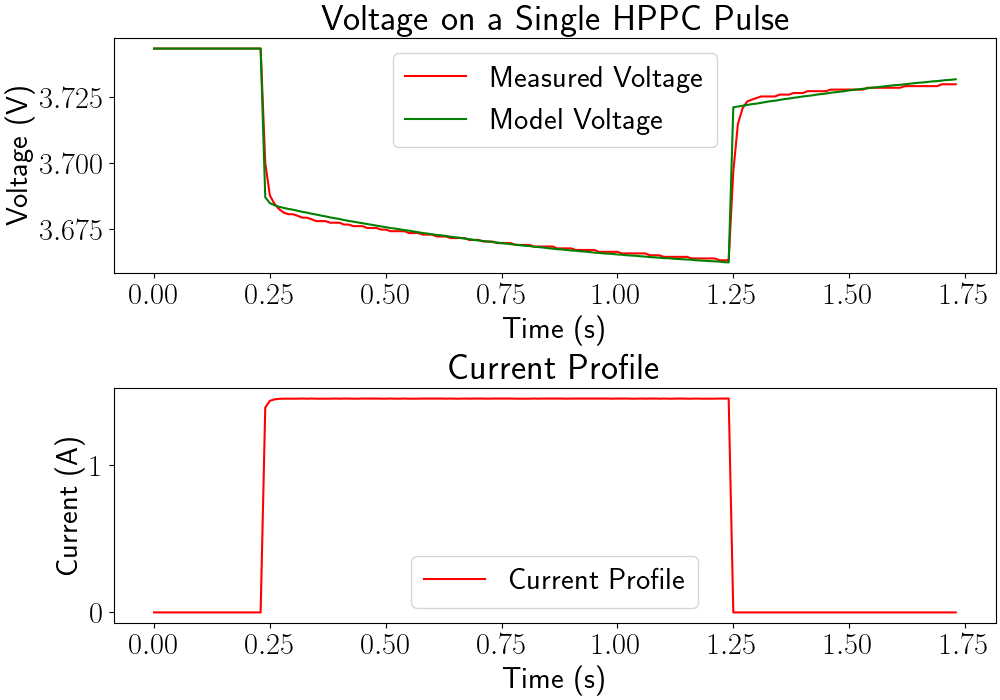
\includegraphics[width=0.6\linewidth]{figures/hppc-pulse.png}
    \caption{HPPC Pulse}
    \label{fig:hppc-pulse}
  \end{figure}

  Empirically, we know that a battery's voltage output looks roughly

  \begin{figure}[H]
    \centering
    \inputtikz{ecm-model}
    \caption{
      The Thevenin equivalent circuit model (ECM) with parameters $R_0 \in \R^+$, $R_1 \in \R^+$ and $C_1 \in \R^+$ and $V_{\rm OC} \in \R^+$ the \textit{open circuit voltage} which behaves according to a function $V_{\rm OC}(s, h, T)$ dependent on $s$, $h$ and $T$.
    }
    \label{fig:ecm}
  \end{figure}

  Kirchhoff's law further tells us that the currents $I_{R1} \in \R$ and $I_{C1} \in \R$ add up to the total current $I = I_{R1} + I_{C1}$, and that the voltages $V_0 \in \R$, $V_1 \in \R$ and $V_{\rm OC}$ sum up to $V = V_0 + V_1 + V_{\rm OC}$.
  The capacitor behaves according to $I_{C1} = C_1 \frac{\dd V_1}{\ddt}$, while the resistors follow Ohm's law $V_0 = R_0 I$ and $V_1 = R_1 I_{R1}$.

  \subsection{Battery in an Electric Vehicle (EV)}
  On a graph $(V_G, E)$ with edges $E = \{AB, AC, ...\} \subseteq V_G \times V_G$ and vertices $V_G = \{A, B, ...\}$, let
  $d_{AB} \in \R^+$ denote the distance between two vertices $A \in V_G$ and $B \in V_G$ (\textcolor{gray}{in meters}),
  $x = x_{AB} \in [0, d_{AB}]$ the progress (current location) on the route from vertex $A$ to $B$ (\textcolor{gray}{in meters}),
  $v := \frac{\ddx}{\ddt}$ denote the current velocity with
  $v_{\rm max, AB} \in \R^+$ the maximum allowed velocity on $AB$ (\textcolor{gray}{in meters per second}).
  Then let
  $T_{\rm env}(x) \in [-273.15, \infty)$ denote the temperature of the environment (\textcolor{gray}{in degrees Celsius}) at location $x$.

  \begin{figure}[H]
    \centering
    \inputtikz{graz-to-munich}
    \caption{Path}
  \end{figure}

  Let $P \in \R$, $P := I \cdot V$ denote the (electrical) power the car draws from the battery (\textcolor{gray}{in Watts}) so $P > 0$ corresponds to discharging the battery.
  This power is to be realised into a mechanical component $P_{\rm motor} \in \R^+$ driving the car forwards, heating for the battery $P_{\rm heat} \in \R^+$, $P_{\rm heat} = c (T - T_{\rm env})$, with $c \in \R^+$ the heat conduction constant describing the relation between the heater and battery, and power dissipation $P_{\rm diss} \in \R^+$.
  While driving, $P = P_{\rm motor} + P_{\rm heat} + P_{\rm diss}$.
  The acceleration of the car $a \in \R$ (\textcolor{gray}{in meters per second squared}), where $a := \frac{\dd v}{\ddt} = \frac{\dd^2 x}{\ddt}$ is decomposed into $a_m \in \R$, which directly impacts $P_{\rm motor}(a_m)$, and the deceleration due to friction (air, etc.) $a_f(v) \in \R^-$, so that in total $a = a_m + a_f$.

  On the graph $(V_G, E)$ there exists a set of EV charging stations $V_{\rm charge} \subseteq V_G$ where $P_{C,\rm charge}$ denotes the possible charging power (\textcolor{gray}{in Watts}) at the charging station vertex $C \in V_{\rm charge}$ with $K_C \in \R^+$ the occuring costs per energy unit (\textcolor{gray}{in Euros per Watt second}) and $t_C \in \R^+$ the charging time per charging station $B$ (\textcolor{gray}{in seconds}).

  \subsection{A Variational Optimisation Problem}
  Given source and destination vertices $A, Z \in V_G$ on the graph $(V_G, E)$, which connected set of edges $E_R \subseteq E$ connecting $A$ to $Z$,
  % battery heating strategy $P_{\rm heat}(x, v, t, s, h, T_{\rm env}, ...)$, $P_{\rm heat} \in \cC(\P)$,
  set of visited charging stations $V_C \subseteq V_{\rm charge}$ and charging times $\{t_C\}_{C \in V_C}$ visited on the route $E_R$, and driving behaviour $a_m(x, v, t, s, h, T_{\rm env}, ...),\, a_m \in \cC^1(\P)$ with $\P$ the parameter space \footnote{to be defined.. TODO} minimises
  \begin{enumerate}
    \item the total travel time $t_{\rm total} := \int_{V_R} \frac{1}{v} \ddx + \sum_{C \in V_C} t_C$,
    \item the total cost of travel $K := \sum_{C \in V_C} P_{C, \rm charge} t_{C} K_C$,
    \item $-N$ where $N$ is the highest possible number of repetitions (commutes from $A$ to $Z$) with the same battery (requiring $h > 0$).
  \end{enumerate}
  Formulated differently, we aim to minimise the functional
  $F \in \cC(\P)^*, F: \cC(\P) \mapsto \R$ where either $F[\chi] = t_{\rm total}$ or $F[\chi] = K$.

  Charging station + street data could be obtained from \href{https://osm.org/}{OpenStreetMap} by calling \\
  \texttt{osmfilter england-latest.o5m \-\-keep="amenity=charging\_station"} \footnote{OSM's public map data may be obtained from \url{https://download.geofabrik.de/}}.

  % \subsection{Notes}
  % \begin{itemize}
  %   % \item
  %   \item Thanks to Nicholas and Zella, we have $R_0$, $R_1$, $C_1$ as functions of $s$, $T$ (and possibly $h$ in the future).
  % \end{itemize}

  % \subsection{Simplifications}
  % Endless possibilities, such as
  % \begin{itemize}
  %   \item $V_G = \{A, B\}$ and $E = \{AB\}$ with some $d_{AB}$ and $v_{\rm max, AB} = \infty$ and $V_C = \{\}$, so only looking at the minimisation of $t_{\rm total}$.
  %   \item $P_{\rm heat} = 0$.
  %   \item $T = T_{\rm env} = \rm const.$ and therefore $P_{\rm heat} = 0$.
  %   \item $P_{\rm diss} = 0$.
  %   \item $a_f = 0$.
  %   \item $h = 1$.
  %   \item $s = \rm const$.
  %   \item etc.
  % \end{itemize}
  % and many more simplifications are possible, which ones do we choose?

  \subsection{Battery Aging}
  \begin{equation*}
    \label{eq:cap}
    Q (t,c,s,I) = Q_{0} - \frac{F_{acycle}(c)}{F_{current}(I)} - F_{cal}
  \end{equation*}
  By $F_{acycle}(c)$ we denote the \textit{Current Agnostic Cycle Degradation Factor} models cycle aging at a single current.
  Also $F_{current}(I)$ represents the \textit{Current Scaling Factor}, a value $0 < F_{current} \leq 1$ that incorporates behaviour where higher currents are worse for cycle aging.
  Finally, $F_{cal}(s,t)$, the \textit{Calendar Degradation Factor}, ages the battery over time and accounts for suboptimal storage in terms of state of charge.

  \begin{figure}[H]
    \centering
    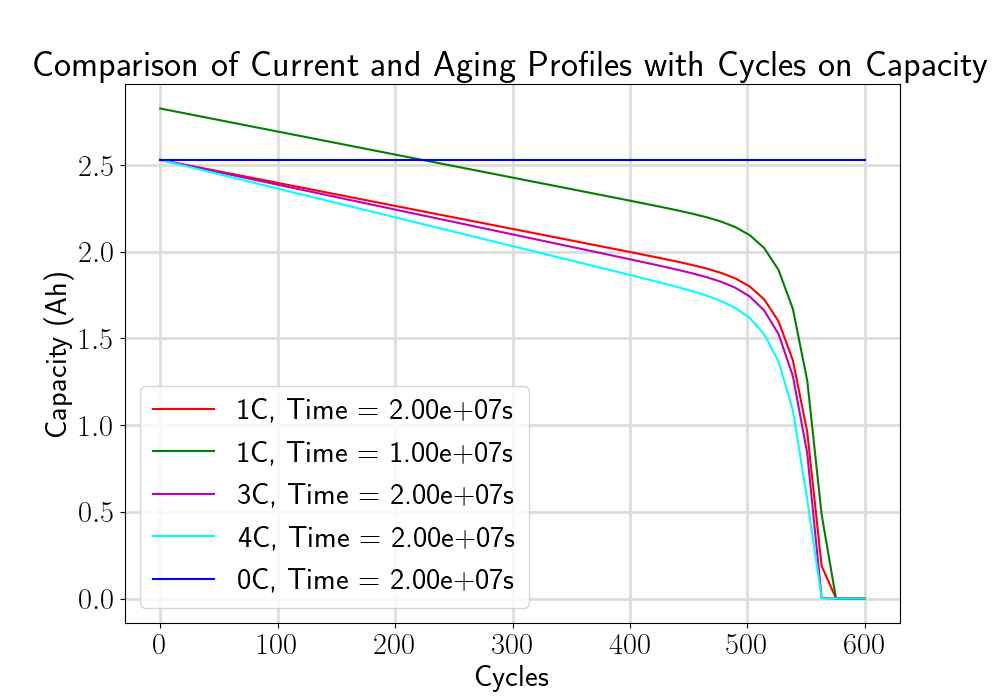
\includegraphics[width=0.7\linewidth]{figures/aging.png}
    \caption{Aging}
    \label{fig:aging}
  \end{figure}

  \begin{figure}[H]
    \centering
    \inputtikz{battery-model-overview}
    \caption{Overview}
    \label{fig:model-overview}
  \end{figure}

  \section{Numerical Simulation of a Car}
  \subsection{Finding ECM Parameters}
  \begin{figure}[H]
    \captionsetup[subfigure]{justification=centering}
    \centering
    \subfloat[Fit of $R_0$ as a function of the SOC ($s$).]{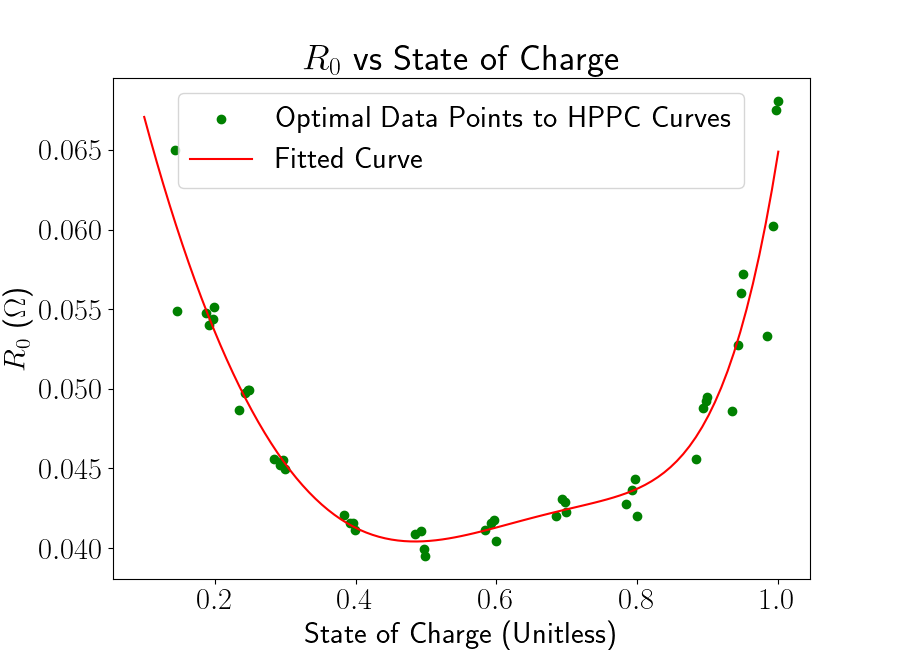
\includegraphics[width=.5\linewidth]{figures/r0fit.png}}\hfill
    \subfloat[Fit of $R_1$ as a function of the SOC ($s$).]{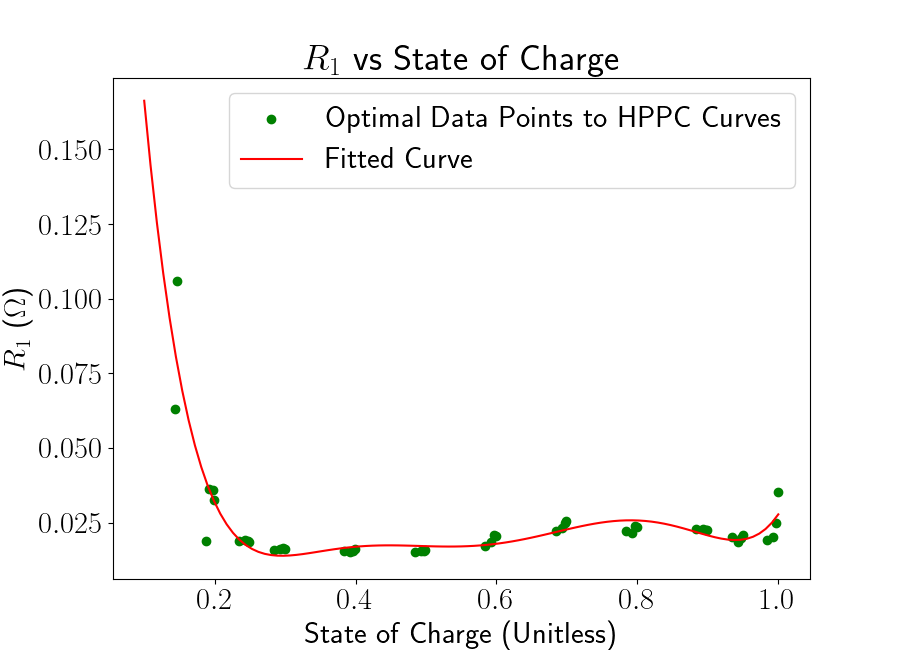
\includegraphics[width=.5\linewidth]{figures/r1fit.png}}\par
  \end{figure}

  \subsection{Forward Euler Simulation}

  \section{Metropolis-Hastings and A-Star}
  \begin{definition}{Undirected Graph}{undirected-graph}
    A graph $G = (V, E)$ with vertices $V$ and edges $E \subseteq V \times V$ is undirected if and only if $(v_i, v_j) \in E \Rightarrow (v_j, v_i) \in E \quad \forall\; v_i, v_j \in V$.
  \end{definition}

  \subsection{Shortest Path Finding}
  The graph data was retrieved using OSMNX \parencite{osmnx} which itself is built on NetworkX \parencite{networkx}.

  \subsection{Monte-Carlo Optimisation}
  Optimise a large problem (huge state-space). Metric: Time! Could be anything.
  $\Rightarrow$ Use Monte-Carlo Markov Chain Methods!
  Slightly perturb the route using a specific alteration technique.
  Metropolis-Hastings updates the state (route) based on $$p_{\rm accept} = \min\left(1, \e^{-\beta (T_{\rm next} - T_{\rm current})}\right)\,, \quad \text{ with } \beta \in \R^+ \text{ a transition factor} \,.$$
  Does a full numerical simulation of the drive. Stop to charge?
  Explore the state-space to some extent, and return the best route!
  Larger scales / maps (e.g. England) are not a problem!

  \begin{minted}{python}
newRoute = self.simulator.batgraph.perturbRoute(self.route)
delta = self.measureRoute(newRoute) - self.testedRoutes[self.route]
acceptanceProbability = min(1, math.exp(-delta / self.temperature))
if random.random() < acceptanceProbability:
    self.route = newRoute
    print(f"Accepted new route {newRoute} with delta: {delta:.2f}. Total: {self.testedRoutes[newRoute]:.2f}.")
else:
    print(f"Rejected route {newRoute} with delta: {delta:.2f}.")
  \end{minted}

  \subsection{Special Case: Granny's House}
  \begin{figure}[H]
    \centering
    \inputtikz{grannys-house}
    \caption{The exemplary problem ``Granny's House'', a special case of Problem (TODO).}
  \end{figure}

  \subsection{Routing in Jericho}
  \begin{figure}[H]
    \centering
    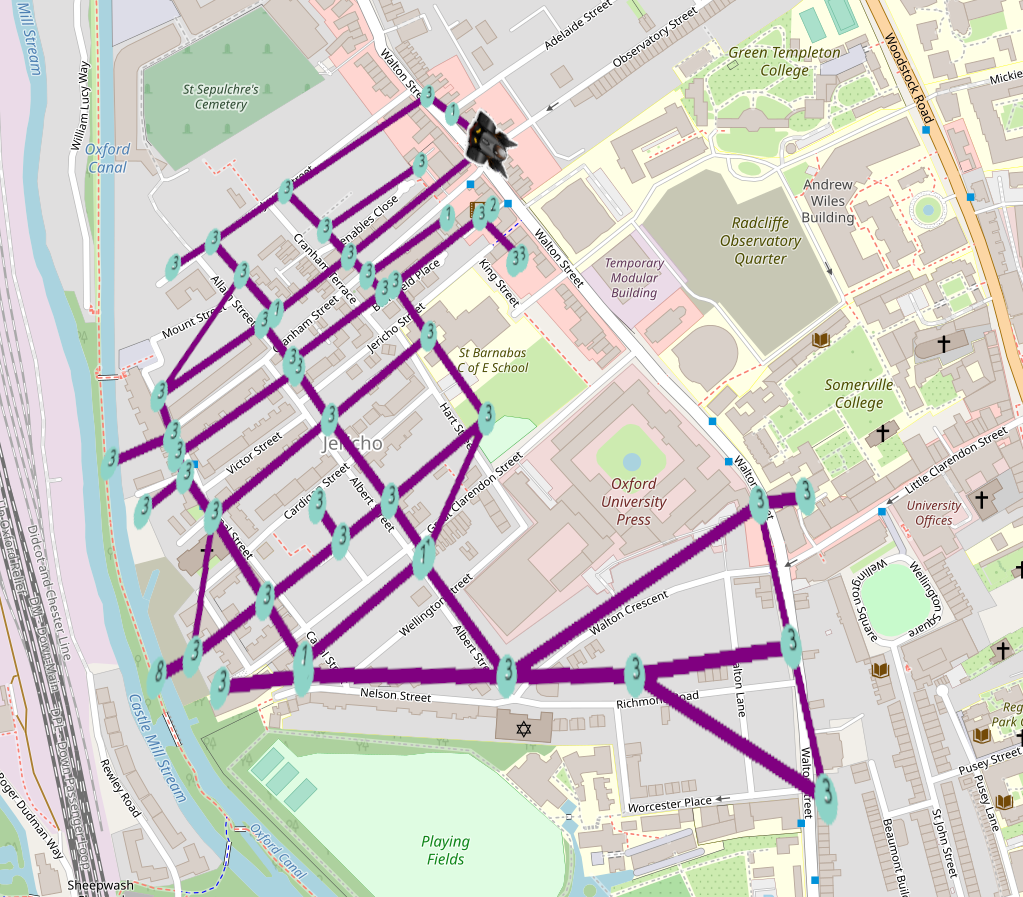
\includegraphics[width=0.6\linewidth]{figures/jericho.png}
    \caption{Overlay of the routing graph on a map of Jericho \parencite{osm}, without adjusting for the Merkator projection, which leads to a slightly skewed appearance. The underlying data is exactly the same.}
  \end{figure}

  \section{Conclusion}

  \pagebreak
  \printbibliography

  \pagebreak
  \appendix
  \section{Simulation Code}
  \inputminted{python}{../simulator/batmobile.py}
\end{document}
